\chapter{Using \corry as Online Monitor}

Reconstructing test beam data with \corry does not require many dependencies and is usually very fast due to efficient data handling and fast reconstruction routines.
It is therefore possible to directly perform a full reconstruction including tracking and analysis of the DUT data during data taking.
On Linux machines this is even possible on the data currently recorded since multiple read pointers are allowed per file.

The \corry framework comes with an online monitoring tool in form of a module for data quality monitoring and immediate feedback to the shifter.
The \command{OnlineMonitor} is a relatively simple graphical user interface which displays and updates histograms and graphs produced by other modules during the run.
It should therefore be placed at the very end of the analysis chain in order to have access to all histograms previously registered by other modules.

\begin{figure}[tbp]
        \centering
        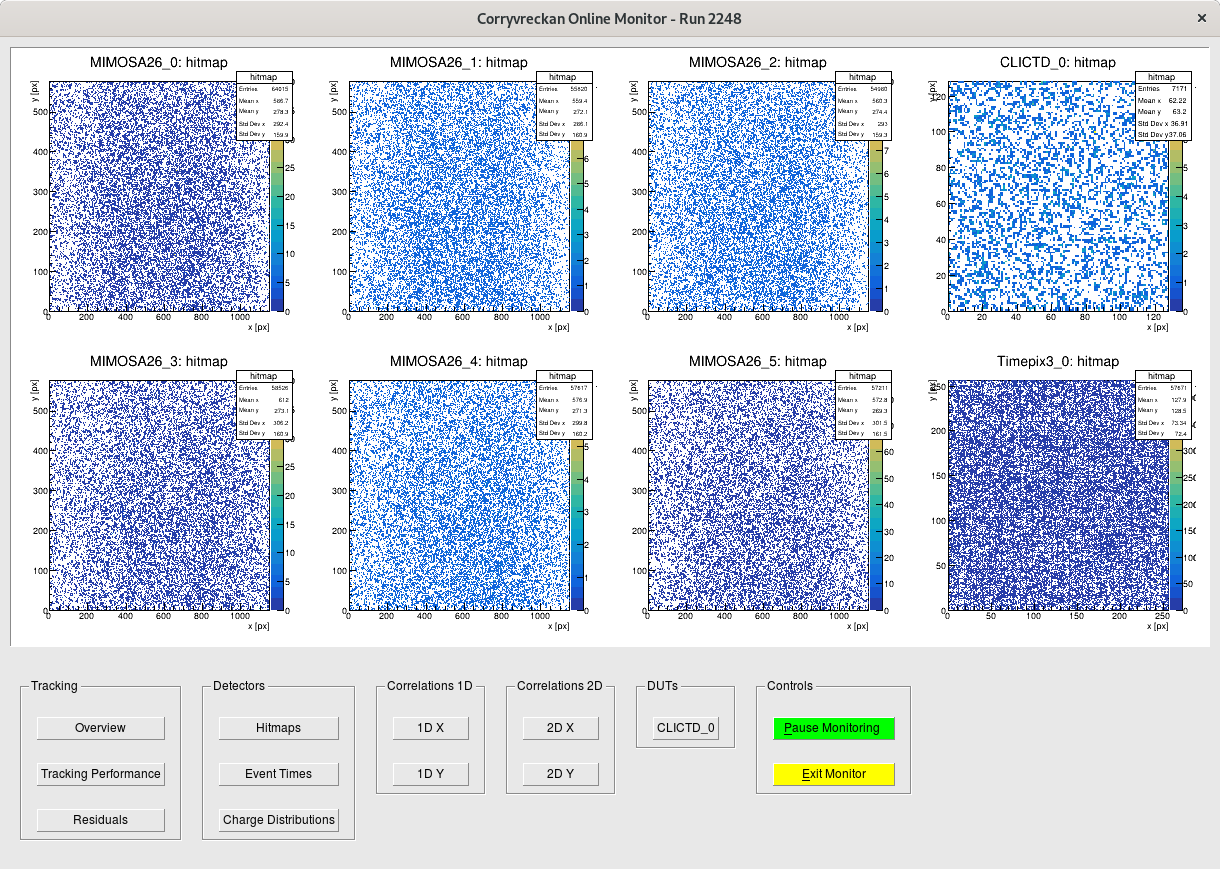
\includegraphics[width=0.9\textwidth]{onlinemon.png}
        \caption{Screenshot of the OnlineMonitor module displaying reconstruction histograms during the \corry run.}
        \label{fig:onlinemon}
\end{figure}

A screenshot of the interface is displayed in Figure~\ref{fig:onlinemon}, showing histograms from the reconstruction of data recorded with the setup presented in Section~\ref{sec:reco_mixedmode}.
The histograms are distributed over several canvases according to their stage of production in the reconstruction chain.
It is possible to add histograms for all registered detectors through the \parameter keyword in the configuration.
Histograms only from all detectors marked as device under test can be added by placing \parameter in the histogram path.

The module has a default configuration which should match many reconstruction configurations, but each of the canvases and histograms can be freely configured as described in the documentation of the \command{OnlineMonitor} in Section~\ref{onlinemonitor}.
